\documentclass[
    11pt,               % KOMA default
    a4paper,            % DIN A4
    %twoside,            % Zweiseitig
%     onside,
    headsepline,        % Linie unter der Kopfzeile
    foodsepline,        % Linie �ber Fussnote
    %automark,           % Kolumnentitel lebendig
    %pointlessnumbers,   % Keinen Punkt hinter die letzte Zahl
                        % eines Kapitels (auch bei Anhang)
%     openleft,           %
    %openright,
    cleardoubleplain,   %
    %abstracton,         %
    %idxtotoc,           % Index soll im Inhaltsverzeichnis auftauchen
    liststotoc,         %
    bibtotoc,           %
    %parskip            % parskip-, parskip*, parskip+
]%{scrreprt}
{article}

%\usepackage[latin1]{inputenc}
\usepackage[utf8]{inputenc}
\usepackage{ngerman}
\usepackage{graphicx}
\usepackage{subfigure}
\usepackage{float}
\usepackage{listings}
\usepackage{color}
\usepackage{tabularx}
\usepackage{hyperref}

\newcommand{\HRule}{\rule{\linewidth}{0.4mm}}

\begin{document}
\begin{center}
	
\includegraphics[scale=0.8]{hszg_logo.png}\\
	\vspace*{2cm}
	%\Large
	%\textbf{Fakultät}\\
	%\textbf{Elektrotechnik und Informatik}\\
	%\vspace*{2cm}
	\Huge
	\textbf{Belegarbeit}\\
	\Large
	\vspace*{2cm}
	\textbf{Durchführung einer Bedrohungs- bzw. Risikoanalyse für Fallbeispiele}\\
	\vspace*{1cm}
	
	\vfill
	\normalsize
	\newcolumntype{x}[1]{>{\raggedleft\arraybackslash\hspace{0pt}}p{#1}}
	\begin{tabular}{x{6cm}p{7.5cm}}
		\rule{0mm}{5ex}Kucera, Adam & {Matr.-Nr.:} 202549\\
		\rule{0mm}{5ex}Krause, Andre & {Matr.-Nr.:} 46932\\
		\rule{0mm}{5ex}Leuschner, Jens & {Matr.-Nr.:} 46932\\
		\rule{0mm}{5ex}Mack, Tobias & {Matr.-Nr.:} 46932\\
		\rule{0mm}{5ex}Michel-Suarez, Maria Belen & {Matr.-Nr.:} 209782\\
		\rule{0mm}{5ex}Müssig, Daniel & {Matr.-Nr.:} 200304\\
		\rule{0mm}{5ex}Riedel, Robert & {Matr.-Nr.:} 46932\\
		\rule{0mm}{5ex}Wollstein, Romano & {Matr.-Nr.:} 46932\\
		\rule{0mm}{5ex}Zoeke, Robert & {Matr.-Nr.:} 200074\\

		\rule{0mm}{5ex}\textbf{Abgabedatum:} & 1.12.2014 \\ 
	\end{tabular} 
\end{center}
\section*{Abstract}
Jüngste Ereignisse, bei denen Millionen Daten von Nutzern aus Online-Systemen gestohlen wurden, zeigen, dass die Bedeutung von Risikoanalysen und die Einrichtung von Schutzmaßnahmen stetig zunehmen. Gerade durch komplexer werdende Systeme und Software sowie die Globalisierung sehen sich viele Unternehmen immer stärkeren Bedrohungen ausgesetzt, die ohne eine durchdachte Sicherheitsstrategie viel Schaden anrichten können. 
\\
\\
In dieser Arbeit wird eine solche Bedrohungs- und Risikoanalyse exemplarisch für zwei Fallbeispiele mit Hilfe eines geeigneten Tools durchgeführt. Weiterhin wird die UML als eine mögliche Alternative zur Darstellung der Analyse untersucht. Außerdem findet eine kritische Betrachtung des eingesetzten Tools zur Analyse statt, bei der die Schwächen der Modelingsoftware aufgezeigt werden.

\newpage
\pagestyle{empty}
\pdfbookmark{\contentsname}{toc}\tableofcontents
\thispagestyle{empty}
\pagestyle{plain}

\setcounter{section}{0}
\pagenumbering{arabic}

\section{Einleitung}
Im Folgenden soll ein Überblick über den Inhalt dieses Belegs gegeben werden. Weiterhin wird der Ablauf des Projektes skizziert und die Aufteilung der Arbeit in Gruppen erläutert.

\subsection{Bedrohungs- und Risikoanalyse}
Jüngste Ereignisse wie der Sony-Skandal von 2011, bei dem es unbekannten Angreifern gelang, in das Online-Netzwerk PlayStation Network (PSN) einzudringen und Daten von rund 77 Millionen Nutzern zu stehlen, zeigen, dass auch große Unternehmen bei der Umsetzung eines umfassenden und angemessenen Sicherheitskonzeptes nicht alle möglichen Bedrohungen bedacht zu haben scheinen. Sony wurde daraufhin zu einer Strafzahlung von 300.000 Euro verurteilt. Somit entstand dem Unternehmen durch diesen Vorfall nicht nur ein wirtschaftlicher Schaden, auch der Imageverlust ist ein nicht zu ignorierender Faktor in dieser Angelegenheit, besonders durch die Tatsache, dass dieser Angriff hätte verhindert werden können. 
\\
\\
Gerade durch die immense Ausbreitung des Internets und der zunehmenden Menge an Daten, die in digitaler Form verschickt oder gespeichert werden, sind auch kleinere Unternehmen gezwungen, sich vor bestehenden Risiken zu informieren und gegebenenfalls Gegenmaßnahmen einzuleiten. Das Risikomanagement bildet dabei die Grundlage, um ein umfassendes Sicherheitskonzept, angepasst an die jeweilige Situation des betrachteten Objektes, zu erstellen und einzuführen. Die Bedrohungs- und Risikoanalyse ist ein wichtiger Baustein des Risikomanagements und dient hauptsächlich zur Identifizierung und Bewertung der möglichen Gefährdungen. Solche können zum Beispiel aktive Angriffe sein, bei denen der Angreifer Sicherheitslücken ausnutzt oder Passwörter per Brut-Force Attacken ausspäht. Aber auch Datenverlust durch höhere Gewalt wie Brand oder Hochwasser können die Integrität des bestehenden Systems gefährden. Menschliches Versagen oder ungeschulte Mitarbeiter sind ebenfalls wichtige Faktoren, die betrachtet und eingeschätzt werden müssen.

\subsection{Projektaufgabe}
Im Rahmen des Moduls "IT-Sicherheitsmanagement" im Wintersemester 2014/15 an der Hochschule Zittau/Görlitz Fachbereich Informatik wurde ein Projekt mit dem Inhalt einer solchen Bedrohungs- und Risikoanalyse durchgeführt. 

\subsection{Ablauf}

\subsection{Vorgehensweise}

\subsection{Aufteilung}
\begin{table}[H]
	\sffamily
	\caption{Aufgabenverteilung}
	\tabulinesep = 1mm %bringt die Reihen etwas weiter auseinander, angenehmer zu lesen
	\centering
		\begin{tabu} to 0.9\textwidth {| X[1.5] | X[3] |}
		\hline
		\textbf{Name} & \textbf{Aufgabe}\\
		\hline 
		Kucera, Adam & \\
		\hline
		Krause, Andre & Kapitel Einleitung\\
		\hline
		Leuschner, Jens & \\
		\hline
		Mack, Tobias & \\
		\hline
		Michel-Suarez, Maria Belen & \\
		\hline
		Müssig, Daniel & \\
		\hline
		Riedel, Robert & \\
		\hline
		Wollstein, Romano & \\
		\hline
		Zoeke, Robert & Misuse Cases \& Evaluation von Seamonster\\
		\hline
	\end{tabu}
\end{table}


%\section{Security Modeling Tools}

Die Anforderungen für die Auswahl der Werkzeuge zur Sicherheitsmodellierung umfassen ein \textit{Systemmodell}, ein \textit{Bedrohungsmodell} und 
damit verbundene \textit{Sicherheitseigenschaften}~\cite{bau2011security}.

Das \textit{Systemmodell} definiert das Verhalten des Systems bei unbeabsichtigten und beabsichtigten Eingaben.
Dabei beruht das Modell auf Anforderungen und Entwurfsspezifikationen oder Quellcoderevisionen.

Beim \textit{Bedrohungsmodell} werden die Ressourcen mit den jeweiligen Zugriffen oder externen Eingriffen darauf festgelegt.
So kann zum Beispiel bei einem Angriff auf das Betriebssystem mit bösartigem Code ein Nutzerprozess manipuliert werden. Der Angreifer ist 
jedoch nicht in der Lage, den Kernel des Betriebssystems zu ändern.
Ein weiteres Beispiel stellt einen Netzwerkangriff dar, bei dem auf Netzwerknachrichten zugegriffen wird, jedoch kein Zugriff auf den internen Zustand
des Host möglich ist.

Die \textit{Sicherheitseigenschaften} legen die zu schützenden Eigenschaften fest.

\subsection{Kriterien}
Das zu verwendende Programm soll dem Nutzer die bestmögliche Un\-ter\-stüt\-zung geben, um eine \textit{Risiko}- bzw. eine \textit{Bedrohungsanalyse} durchzuführen.
Weiterhin soll das Programm durch den Nutzer leicht und intuitiv zu bedienen sein.
\begin{itemize}
\item Eine grafische Benutzeroberfläche zur Visualisierung der Modelle ist dabei unverzichtbar.

\item Ebenfalls sollte die Modellierung durch die bekannte und bewährte \textit{Unified Modeling Language~(UML)} erfolgen.

\item Für ein flexibles Arbeiten ist eine nicht-kommerzielle und platt\-form\-un\-ab\-häng\-ige Lösung unausweichlich.

\item In Bezug auf die \textit{Bedrohungs}- und \textit{Risikoanalyse} sollte der Nutzer durch integrierte Artefakte in der Lage sein \textit{Attack-Trees} und\\ \textit{MisUseCases}
abzubilden.

\item Automationen zur Erstellung von Risikomatrizen und zur Analyse hinsichtlich der Kosten und Eintrittswahrscheinlichkeiten sollte das Programm bereitstellen.
\end{itemize}

\pagebreak

\subsection{SecurITree}

Tabelle~\ref{tab:secitree} zeigt die Eigenschaften und den Funktionsumfang des Programms \textit{SecurITree}.
Das plattformübergreifende Programm \textit{SecurITree} eignet sich für die Erstellung von \textit{Attack-Trees} und für eine einfache \textit{Bedrohungs}- und \textit{Risikoanalyse}.

Der Hersteller \textit{Amenza} bietet die Möglichkeit das Tool als Testversion zu evaluieren, wobei eine \textit{Evaluationslizenz} benötigt wird. Für die standardmäßige Verwendung kann \textit{SecurITree} für 10.500 USD käuflich erworben werden. Somit widerspricht \textit{SecurITree} den Kriterien in dem Punkt der freien Verfügbarkeit.

\begin{table}[htbp]
\caption{Eigenschaften von SecurITree}
\label{tab:secitree}
\renewcommand{\arraystretch}{1.5}
\begin{tabularx}{\textwidth}{ l !{\color{white}\vrule}  X }
%\hline
\rowcolor{mydarkblue}  \multicolumn{2}{|c|}{ \textbf{ \color{white}{SecurITree}} } 					\\
\arrayrulecolor{white}\hline
\rowcolor{mylightblue}Tool Kategorisierung 	& Security Modeling Tools	\\
\arrayrulecolor{white}\hline
\rowcolor{mylightgray}Aktuelle Version  		& 2.5 								\\
\arrayrulecolor{white}\hline
\rowcolor{mylightblue}Beschreibung				& \textit{SecurITree} ist ein einfach zu nutzendes Softwarepaket für \textit{Attack Tree} basierte Bedrohungs/Risikoanalyse.
Es ist lauffähig auf Windows, Apple und Linux Plattformen.
 		\linebreak \linebreak Kostenpflichtig							\\
\arrayrulecolor{white}\hline 
\rowcolor{mylightgray}Architektur				& Plattformübergreifend \\
\arrayrulecolor{white}\hline
\rowcolor{mylightblue}Funktionsumfang		& \begin{itemize}
										\item  Bedrohungsbäume
										\item Bedrohungsanalyse
										\item Risikoanalyse
										\item logische Bäume
									\end{itemize}\\
\arrayrulecolor{white}\hline
\rowcolor{mylightgray} Webseite		&		\url{https://www.amenaza.com} \\
\arrayrulecolor{white}\hline
\end{tabularx}
\end{table}


\subsection{Seamonster}
Seamonster (Tabelle~\ref{tab:seamonster}) ist ein Freeware-Tool um Bedrohungsmodelle zu erstellen. Es basiert auf einer Notation, die sich bei erfahrenen Sicherheitsexperten bewährt hat. 

In Seamonster steht neben \textit{Vulnerabilty cause graphs}, \textit{Security Activity graphs} und \textit{Security Modellen}, vor allem die Erstellung von \textit{Misuse-Cases} und \textit{Attack-Trees} im Vordergrund.

Die Defizite von Seamonster liegen bei den Kriterien der Risikomatrix und der Analyse, die nicht abgedeckt werden.

\begin{table}[h!tbp]
\renewcommand{\arraystretch}{1.5}
\caption{Eigenschaften von Seamonster}
\label{tab:seamonster}
\begin{tabularx}{\textwidth}{ l !{\color{white}\vrule}  X }
%\hline
\rowcolor{mydarkblue}  \multicolumn{2}{|c|}{ \textbf{ \color{white}{SeaMonster}} } 					\\
\arrayrulecolor{white}\hline
\rowcolor{mylightblue}Tool Kategorisierung 	& Security Modeling Tools	\\
\arrayrulecolor{white}\hline
\rowcolor{mylightgray}Aktuelle Version  		& 5.0 								\\
\arrayrulecolor{white}\hline
\rowcolor{mylightblue}Beschreibung				& SeaMonster ist ein \textit{Security Modeling Tool} für Bedrohungsmodelle. Es unterstützt Notationen welche von 
Sicherheitsexperten und Analysten verwendet werden. SeaMonster unterstützt beim erstellen von \textit{Attack Trees} und \textit{Missue Cases}.						\linebreak \linebreak Gratis			\\
\arrayrulecolor{white}\hline
\rowcolor{mylightgray}Architektur				& Die Architektur von SeaMonster basiert auf \textit{Eclipse}, welches mit Plugins erweitert werden kann. Die zugehörigen Plugins sind 
								   \textit{Graphical Modeling Framework (GMF)}, das \textit{Eclipse Modeling Framework (EMF)} und das 
								  \textit{Graphical Editing Framework (GEF)} \\
\arrayrulecolor{white}\hline
\rowcolor{mylightblue}Funktionsumfang		& \begin{itemize}
										\item 2D Diagramme
										\item UML
										\item Missue Cases 
										\item Attack Trees 
										\item Vulnerability cause Graphs 
										\item Security Activity Graphs 
										\item Security model 
									\end{itemize}\\
\arrayrulecolor{white}\hline
\rowcolor{mylightgray} Webseite		&		\url{http://seamonster.wiki.sourceforge.net/} \\
\arrayrulecolor{white}\hline
\end{tabularx}
\end{table}

\pagebreak
\subsection{CORAS}
Tabelle~\ref{tab:coras} zeigt die Eigenschaften des \textit{CORAS-Tools}.
Mit dem frei verfügbaren Diagrammeditor \textit{CORAS} wird dem Nutzer die Modellierung aller Arten von Diagrammen ermöglicht. Da \textit{CORAS} auf \textit{Eclipse} basiert, ist ein plattformübergreifender Einsatz gewährleistet.  Das Tool unterstützt die Erstellung von 2D-Diagrammen aufbauend auf UML, die modellbasierte \textit{Risikoanalyse}, eine Syntaxprüfung, sowie eine methodenorientierte Analyse.

Schwachstellen des Tools sind eine fehlende \textit{Attack-Tree-Modellierung}, eine automatisierte Analyse und das Fehlen von \textit{Risiko}- bzw. \textit{Bedrohungsmatrizen}.


\begin{table}[htbp]
\renewcommand{\arraystretch}{1.5}
\caption{Eigenschaften von CORAS}
\label{tab:coras}
\begin{tabularx}{\textwidth}{ l !{\color{white}\vrule}  X }
%\hline
\rowcolor{mydarkblue}  \multicolumn{2}{|c|}{ \textbf{ \color{white}{CORAS}} } 					\\
\arrayrulecolor{white}\hline
\rowcolor{mylightblue}Tool Kategorisierung 	& Security Modeling Tools	\\
\arrayrulecolor{white}\hline
\rowcolor{mylightgray}Aktuelle Version  		& 1.1 								\\
\arrayrulecolor{white}\hline
\rowcolor{mylightblue}Beschreibung				& Das \textit{CORAS tool} ist ein Diagrammeditor, welcher frei verfügbar ist.
Das Tool wurde für die Unterstützung von \textit{on-the-fly} Modellierungen aller Arten von CORAS Diagrammen entworfen.
 		\linebreak \linebreak Gratis							\\
\arrayrulecolor{white}\hline
\rowcolor{mylightgray}Architektur				& Plattformübergreifend \\
\arrayrulecolor{white}\hline
\rowcolor{mylightblue}Funktionsumfang		& \begin{itemize}
										\item  2D Diagramme
										\item UML
										\item modellbasierte Risikoanalyse
										\item Reporting
										\item Methodenorientierte Analyse
									\end{itemize}\\
\arrayrulecolor{white}\hline
\rowcolor{mylightgray} Webseite		&		\url{http://coras.sourceforge.net} \\
\arrayrulecolor{white}\hline
\end{tabularx}
\end{table}

\pagebreak
\subsection{Microsoft Threat Modeling Tool}
Die Eigenschaften von \textit{Microsofts Threat Modeling Tool} sind in Tabelle~\ref{tab:mstool} zu sehen.
Das Programm unterstützt Softwareentwickler bei der Erstellung und \textit{Analyse} von \textit{Bedrohungsmodellen} und deren Analyse. Dabei ist das Tool unter Microsoft Windows lauffähig und steht zum freien Download zur Verfügung.

Da das Tool speziell für eine Unterstützung während des Softwareentwicklungsprozesses entwickelt wurde, ist das Tool für die Modellierung von allgemeinen Sicherheitssystemen ungeeignet.

\begin{table}[htbp]
\renewcommand{\arraystretch}{1.5}
\caption{Eigenschaften von Microsofts Threat Modeling Tool}
\label{tab:mstool}
\begin{tabularx}{\textwidth}{ l !{\color{white}\vrule}  X }
%\hline
\rowcolor{mydarkblue}  \multicolumn{2}{|c|}{ \textbf{ \color{white}{Microsoft Threat Modeling Tool}} } 					\\
\arrayrulecolor{white}\hline
\rowcolor{mylightblue}Tool Kategorisierung 	& Security Modeling Tools	\\
\arrayrulecolor{white}\hline
\rowcolor{mylightgray}Aktuelle Version  		& 1.0								\\
\arrayrulecolor{white}\hline
\rowcolor{mylightblue}Beschreibung				&  Das \textit{SDL Threat Modeling Tool} ist das erste Bedrohungsmodellierung-Tool, welches nicht nur für Sicherheitsexperten entwickelt wurde. Die Bedrohungsmodellierung wird durch eine Führung bei dem Erstellen und Analysieren des Bedrohungsmodells für Entwickler vereinfacht.
		\linebreak \linebreak Gratis							\\
\arrayrulecolor{white}\hline
\rowcolor{mylightgray}Architektur				& Windows \\
\arrayrulecolor{white}\hline
\rowcolor{mylightblue}Funktionsumfang		& \begin{itemize}
										\item  2D Diagramme
										\item Bedrohungsanalyse und Modellierung
									\end{itemize}\\
\arrayrulecolor{white}\hline
\rowcolor{mylightgray} Webseite		&		\url{http://www.microsoft.com/en-us/download/details.aspx?id=42518} \\
\arrayrulecolor{white}\hline
\end{tabularx}
\end{table}

\subsection{Security Requirements Modeling Tool}
Das \textit{Security Requirements Modeling Tool} (Tabelle~\ref{tab:sts}) ist eine Freeware zur Modellierung und Analyse von Sicherheitskritischen Systemen. Dabei wird auf eine herstellereigene Modellierungssprache  (STS-ml) gesetzt. Des weiteren basiert das Tool auf dem \textit{Eclipse RCP Framework}, wodurch  plattformübergreifendes Arbeiten gegeben ist. Weitere Features  sind die Dokumentgenerierung, die Sicherheitsanforderungsanalyse und eine automatisierte Analyse hinsichtlich der Wohlgeformtheit und der Modellsyntax.

Da die Sprache \textit{STS-ml} anders als UML keine standardisierte Sprache in der Welt der Modellierung darstellt, ist hierbei eine längere Einarbeitungszeit notwendig. Weitere negative Punkte des Tools sind die fehlende Unterstützung zur Erstellung von \textit{Misuse-Cases} und \textit{Bedrohungsmatrizen}, sowie die nicht vorhandene automatische Analyse bezüglich der Kosten und der Auftrittswahrscheinlichkeiten.

\begin{table}[htbp]
\renewcommand{\arraystretch}{1.5}
\caption{Eigenschaften vom  Security Requirements Modeling Tool}
\label{tab:sts}
\begin{tabularx}{\textwidth}{ l !{\color{white}\vrule}  X }
%\hline
\rowcolor{mydarkblue}  \multicolumn{2}{|c|}{ \textbf{ \color{white}{Security Requirements Modeling Tool}} } 					\\
\arrayrulecolor{white}\hline
\rowcolor{mylightblue}Tool Kategorisierung 	& Security Modeling Tools	\\
\arrayrulecolor{white}\hline
\rowcolor{mylightgray}Aktuelle Version  		& 2.0								\\
\arrayrulecolor{white}\hline
\rowcolor{mylightblue}Beschreibung				&  Das \textit{STS-Tool} ist das Modellierungs- und Analyse-Tool, welches auf der \textit{STS-Modeling Language (STS-ml)} aufbaut. Es ist eine eigenständige Applikation, welche auf dem \textit{Eclipse RCP Framework} basiert. 		\linebreak \linebreak Gratis							\\
\arrayrulecolor{white}\hline
\rowcolor{mylightgray}Architektur				& Plattformübergreifend \\
\arrayrulecolor{white}\hline
\rowcolor{mylightblue}Funktionsumfang		& \begin{itemize}
										\item  2D Diagramme
										\item STS-ml 
										\item Dokumentgenerierung
										\item Sicherheitsanforderungsanalyse
										\item automatisierte Analyse hinsichtlich Wohlgeformtheit und Syntax
									\end{itemize}\\
\arrayrulecolor{white}\hline
\rowcolor{mylightgray} Webseite		&		\url{http://www.sts-tool.eu} \\
\arrayrulecolor{white}\hline
\end{tabularx}
\end{table}

\pagebreak
\subsection{Auswertung der Tools}
Nach dem Betrachten aller Eigenschaften der zuvor beschriebenen Tools ergibt sich das Fazit, dass keines der Programme alle geforderten 
Eigenschaften abdeckt.
So wäre \textit{SecurITree} im Vergleich zu den anderen Tools die beste Wahl, ist jedoch durch den kommerziellen Vertrieb für die von 
uns geforderten Anforderungen untragbar.

Die zweite Wahl fällt auf \textit{Seamonster}, da es im Vergleich zu den anderen Tools die wenigsten Defizite aufweist.
Damit ist \textit{Seamonster} für die Bearbeitung des Projekts am besten geeignet.




\section{Vorgehen bei der Risikoanalyse}

Abbildung~\ref{5analysestufen} zeigt schematisch das Vorgehen bei der Risikoanalyse. Es gilt als erstes die zu schützenden \textit{Werte} zu \textit{identifizieren}. Danach ermittelt man die \textit{Bedrohungen}, welche für die vorher ermittelten Werte bestehen. Anschließend müssen die \textit{Schwachstellen} identifiziert werden, durch welche die Bedrohung wirksam werden kann. Anschließend kann man die \textit{Risiken bewerten} mittels der Formel
\\\\
$ Risiko = Bedrohung * Schwachstelle * Wert $
\\\\
und entsprechende \textit{Prioritäten setzten}, was geschützt werden muss. Ist dies geschehen, kann man entsprechende \textit{Gegenmaßnahmen finden}.

\begin{figure}[h]
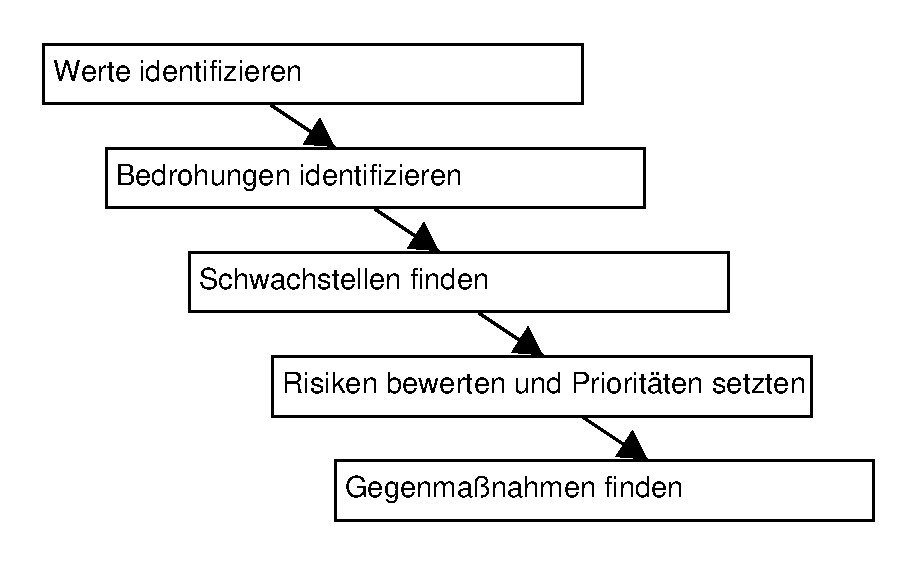
\includegraphics[scale=0.8]{images/5analysestufen.pdf}
\caption{Schematisches Vorgehen bei der Risikoanalyse}
\label{5analysestufen}
\end{figure}

\\

\subsection{Werte identifizieren}
Um die zu schützenden Werte zu identifizieren gibt es mehrere Möglichkeiten. Der einfachste Ansatz ist des, dem Fluss des Geldes zu folgen. Objekte mit einem festen Preis in der Anschaffung können exakt mit Zahlen erfasst werden. Sie sind relativ leicht für die Wiederbeschaffung zu beziffern. 
\section{Schadensberechnung}
%\include{analyse_FBI}

%\include{analyse_FBII}

\section{MisUse Cases}



\section{Evaluation von SeaMonster}

%\section{UML als adäquate Lösung?}
In diesem Abschnitt soll beschrieben werden, in wie weit UML als Alternative zu Tools wie zum Beispiel SeaMonster verwendet werden kann. Dazu sollen die Vor- und Nachteile dieser Lösung aufgezeigt werden. Zum Schluss soll bewertet werden, ob UML zur Risikoanalyse eingesetzt werden sollte oder nicht.

\subsection{Vorteile}
UML ist eine Modellierungssprache, die seit den 1990er Jahren vor allem in der Software Entwicklung eingesetzt wird. Da es bereits seit ca. 25 Jahren und von beinahe jedem Entwickler eingesetzt wird, verfügt UML über viele Tools, die verwendet werden können um UML-Diagramme zu erstellen. Es gibt für jedes Betriebssystem mindestens ein Tool, wobei so gut wie alle sehr leicht zu bedienen sind. Die weite Verbreitung dieser Sprache sorgt vor allem auch dafür, dass sie bereits in der Ausbildung gelernt wird und daher auch von einer breiten Masse verstanden wird.\\
UML umfasst ca. 13 Diagrammarten, was dafür sorgt, dass UML eine große Palette an Modellen unterstützt. Es bietet zum Beispiel die Möglichkeit UseCase-Diagramme zu zeichnen, die den MisUseCase-Diagrammen der Risikoanalyse entsprechen.

\subsection{Nachteile}
Bei der Risikoanalyse werden häufig sehr viele Daten benötigt. Diese alle in ein Diagramm unterzubringen ohne das die Lesbarkeit darunter leidet ist kaum möglich. Gerade auch die Tatsache, das bei der Analyse viele Berechnungen durchgeführt werden müssen mindert die Nutzbarkeit von UML.\\
Außerdem bietet UML auch nur eine begrenzte Menge an Zeichenelementen, wodurch zum Beispiel das Zeichnen von Attack-Trees nicht sinnvoll möglich ist.

\subsection{Bewertung}
Die große Anzahl der Diagrammarten sowie die weite Verbreitung der Sprache sprechen für UML. Jedoch überwiegen die Nachteile, da aufgrund fehlender Zeichenelemente und der Unübersichtlichkeit die Verwendung von UML erschwert wird. Auch fehlt die Verknüpfung zu einer Tabelle, in der weitere Einzelheiten und Anmerkungen festgehalten werden können. Aufgrund der überwiegenden Nachteile, ist von der Verwendung von reinem UML für die Risikoanalyse abzuraten.

%\section{Fazit}
Die Arbeit an diesem Projekt hat vor allem gezeigt, dass es mit unter ziemlich schwierig sein kann, konkrete Bedrohungen für ein Objekt zu finden und diese auch entsprechend zu bewerten. Außerdem ist die Einstufung von Risiken und dem entstehenden Schaden von Unternehmen zu Unternehmen unterschiedlich. Es hat sich gezeigt, dass die Risiken und Bedrohungen oft gleich sind, es aber eine eingehende Analyse benötigt, um den optimalen Sicherheitsprozess für das jeweilige System zu finden.
\\
\\
Bei der Auswahl der Tools zur Unterstützung der Analyse sind schnell Probleme aufgetreten, wie etwa das Fehlen eines umfangreichen Angebots solcher Modelingprogramme. Außerdem bieten Open-Source Programme oft nicht den gewünschten vollen Umfang an Funktionen, wodurch man gewisse Einschränkungen in Kauf nehmen muss. Zwar gibt es auch die Möglichkeit, kommerzielle Software einzusetzen, welche durch einen besseren Support seitens des Herstellers und eines größeren Funktionsumfangs hervorstechen. Es hätte aber in keinem Verhältnis zu den Kosten/Nutzen in diesem knapp sechswöchigen Projekt gestanden, daher viel eine solche Lösung heraus.

%======================================================================
%   Literaturverzeichnis
%======================================================================
\renewcommand{\baselinestretch}{1.13}\normalsize
\markboth{BIBLIOGRAPHY}{BIBLIOGRAPHY}
\renewcommand{\bibname}{BIBLIOGRAPHY}
\bibliographystyle{plaindin}
\selectlanguage{ngerman}
\bibliography{literatur}
\cleardoublepage

%======================================================================
%   Selbstständigkeitserklärung
%======================================================================
\selectlanguage{ngerman}
\section*{Selbstständigkeitserklärung}
\thispagestyle{empty} Hiermit erklären wir, dass wir die vorliegende
Arbeit selbstständig angefertigt, nicht anderweitig zu
Prüfungszwecken vorgelegt und keine anderen als die angegebenen
Hilfsmittel verwendet haben. Sämtliche wissentlich verwendete
Textausschnitte, Zitate oder Inhalte anderer Verfasser
wurden ausdrücklich als solche gekennzeichnet.\\[2ex]

\end{document}